% === Fig. 1: Hero illustration ===
\begin{figure*}[t]
    \centering
    \includegraphics[width=0.96\textwidth]{figures/ai_generated/fig1_hero_pipeline.png}
    \caption{Diagnostic-plus-method overview. In the corrected AFDM evaluation, useful headroom is concentrated in sparse decision-boundary crossings rather than smooth mean-level residual shifts. This motivates a frozen observable bit-level corrector, which improves BER across untouched and shifted regimes while retaining an explicit failure boundary under severe path-count shift.}
    \label{fig:hero_overview}
\end{figure*}

% === Fig. 2: Regime gains ===
\begin{figure}[t]
    \centering
    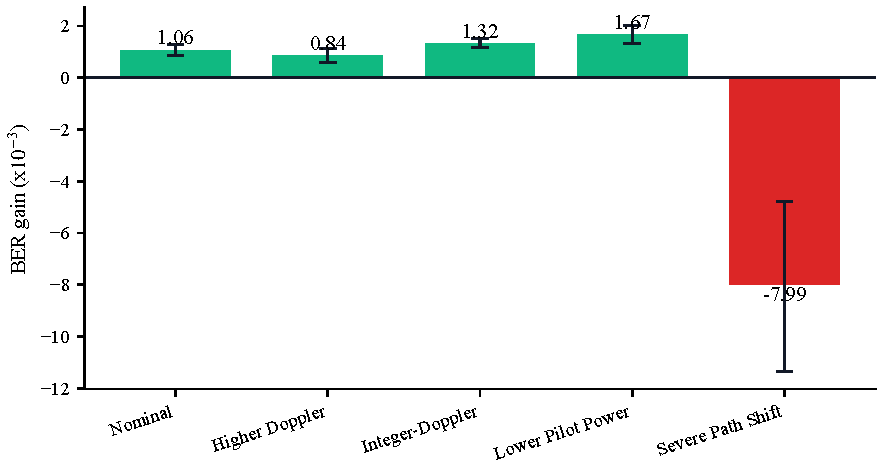
\includegraphics[width=0.48\textwidth]{figures/fig2_regime_gains.pdf}
    \caption{BER gain of the frozen corrector across evaluation regimes. Error bars show paired-bootstrap 95\% confidence intervals. Positive regimes remain above zero, while the severe path-count shift is cleanly negative.}
    \label{fig:regime_gains}
\end{figure}

% === Fig. 3: Packet-level impact ===
\begin{figure}[t]
    \centering
    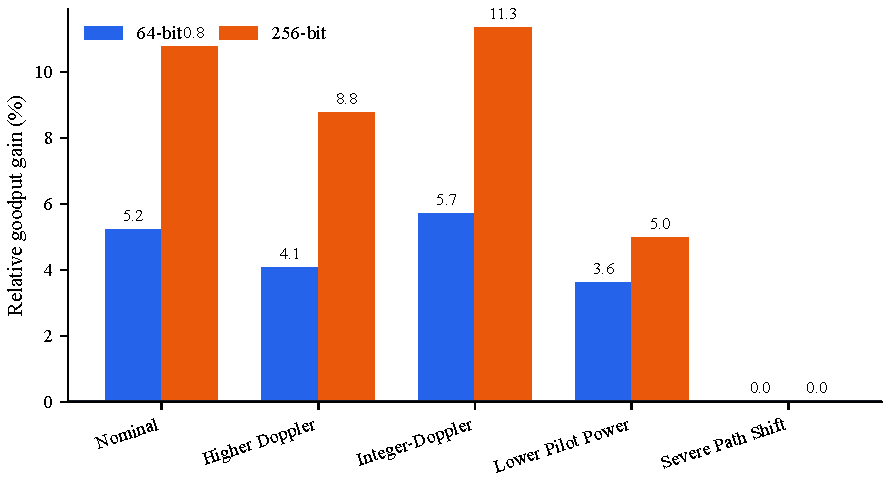
\includegraphics[width=0.48\textwidth]{figures/fig3_system_impact.pdf}
    \caption{Relative goodput gains for 64-bit and 256-bit contiguous packets. Small BER gains can amplify into meaningful endpoint gains in the positive regimes, while the severe path shift loses packet-level benefit.}
    \label{fig:system_impact}
\end{figure}

% === Fig. 4: Feature ablation ===
\begin{figure}[t]
    \centering
    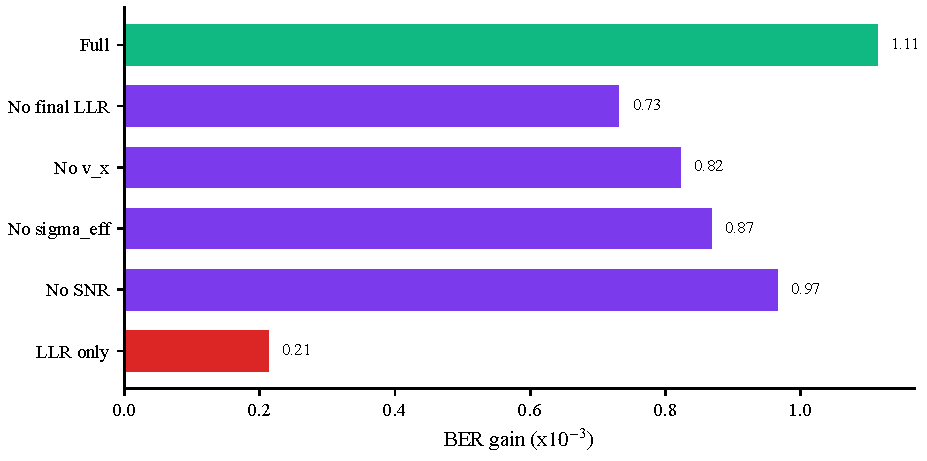
\includegraphics[width=0.48\textwidth]{figures/fig4_feature_ablation.pdf}
    \caption{Feature-group ablation of the frozen corrector. The full observable feature set is strongest, and LLR-only retains only a small fraction of the full gain.}
    \label{fig:feature_ablation}
\end{figure}

% === Table I ===
\begin{table*}[t]
\centering
\caption{Method evolution from failed residual correction to the final frozen direct-bit corrector.}
\label{tab:method_evolution}
\begin{tabular}{p{2.6cm}p{2.8cm}p{3.2cm}p{6.4cm}}
\toprule
Method & Family & Test protocol & Headline outcome \\
\midrule
JointOMPMP & Classical iterative baseline & direct evaluation & historical anchor baseline \\
CurrentJoint & Learned baseline & direct evaluation & base receiver for the final method \\
vx\_recal\_v1 & Detector calibration & corrected same-test-set evaluation & no meaningful BER change \\
distill\_pure\_iter0 & Mean-residual distillation & corrected same-test-set evaluation & headline claim collapses after correction \\
Observable direct-bit corrector & Split-specific probe & split-specific evaluation & gain 6.8359e-04 to 9.2773e-04 \\
Frozen direct-bit corrector & Final method & train-once/test-on-many & nominal gain 1.0590e-03; survives 3 shifts \\
\bottomrule
\end{tabular}
\end{table*}


% === Table II ===
\begin{table*}[t]
\centering
\caption{Claim and scope matrix used to keep the paper aligned with the validated evidence.}
\label{tab:claim_scope}
\begin{tabular}{p{4.2cm}p{5.3cm}p{4.5cm}}
\toprule
Claim & Key evidence & Scope or limitation \\
\midrule
Mean-residual correction is not decision-effective in corrected AFDM evaluation & corrected same-test-set comparison and decision audit & current AFDM joint receiver setting \\
Frozen decision-level correction yields reproducible BER gains & untouched nominal caches, mean gain 1.0590e-03 & train-once/test-on-many inside current simulator family \\
The gain transfers across 3 regime shifts & positive gains under Doppler, integer-Doppler, and rho=0.4 shifts & 10-25 dB, AFDM internal regime shifts \\
The method has an explicit failure boundary & P\_paths=15 regression and negative confidence interval & harsh structural shift breaks the method \\
Small BER gains can be operationally meaningful & 64-bit and 256-bit goodput gains & uncoded contiguous packets with ARQ proxy \\
\bottomrule
\end{tabular}
\end{table*}

